\documentclass[11pt]{scrartcl}

\title{Software Architektur: JBomberman}
\author{Silvan Adrian \\ Fabian Binna \\ Pascal Kistler}
\date{\today{}}

\usepackage[ngerman]{babel}
\usepackage[automark]{scrpage2}
\usepackage{hyperref}
\usepackage{color}
\usepackage[normalem]{ulem}
\usepackage{scrpage2}
\usepackage{graphicx}
\usepackage{tabularx}
\graphicspath{ {./images/} }
\pagestyle{scrheadings}

\clearscrheadfoot
\ihead{
\includegraphics[scale=0.4]{jbomberman}}
\ohead{Projekt: JBomberman}
\ifoot{Software Architektur: JBomberman}
\cfoot{Version: 1.00}
\ofoot{Datum: 01.04.15}
\setheadsepline{0.5pt}
\setfootsepline{0.5pt}

\usepackage{ucs}
\usepackage[utf8]{inputenc}
\usepackage[T1]{fontenc}


\begin{document}
\def\arraystretch{1.5}
\begin{titlepage}
\begin{center}
\vspace{10em}

\includegraphics[scale=2]{jbomberman}
\vspace{10em}
\end{center}
\begin{center}
\huge {Projekt: JBomberman} \\
\huge {Software Architektur}
\end{center}
\begin{center}
\vspace{10em}
\LARGE {Pascal Kistler} \\
\LARGE {Silvan Adrian} \\
\LARGE {Fabian Binna}
\end{center}

\end{titlepage}

\newpage
\section{Änderungshistorie}
\label{sec:Änderungen}

\begin{tabularx}{\linewidth}{l l l l}
\textbf{Datum} & \textbf{Version} & \textbf{Änderung}  & \textbf{Autor} \\
\hline
\textbf{01.04.15} & 1.00 & Erstellung des Dokuments & Gruppe \\
\textbf{05.04.15} & 1.01 & Logische Architektur & Fabian Binna \\
\end{tabularx}

\newpage
\tableofcontents
\newpage

\section{Einführung}
\subsection{Zweck}
Dieses Dokument beschreibt die Software Architektur für das Projekt JBomberman.
\subsection{Gültigkeitsbereich}
Dieses Dokument ist während des ganzen Projekts gültig und wird laufend aktualisiert.
\subsection{Referenzen}
<Liste aller verwendeten und referenzierten Dokumente, Bücher, Links, usw.>
<Referenz auf ein Glossar Dokument, wo alle Abkürzungen und unklaren Begriffe erklärt werden>
<Die Quellen / Referenzen sollten mit dem Word Tool automatisch erstellt werden>
\subsection{Übersicht}
<Übersicht über den restlichen Teil dieses Dokumentes geben und dessen Aufbau erläutern>
 
\section{Systemübersicht}
<Beschreibt die Softwarearchitektur eines Systems und wie sie sich präsentiert (am besten mit einem Bild um eine Übersicht zu ermöglichen) und einzelne Beschreibungen zu den einzelnen Elementen des Systems>
 
\section{Architektonische Ziele \& Einschränkungen}
<Beschreibt die Softwareanforderungen und Objekte, welche einen Einfluss auf die Architektur haben (z.B. Safety, Security, Privacy, Distribution, usw.); Beinhaltet auch eine Beschreibung von Design und Implementationsstrategie, Entwicklungstools, usw.>

\newpage
 
\section{Logische Architektur}
Dieses Package Diagramm zeigt sowol Client, als auch Server. Client und Server sind zwei eigenständige Applikationen, die getrennt ausgeführt werden. Sie verwenden jedoch teilweise die gleichen Packages.

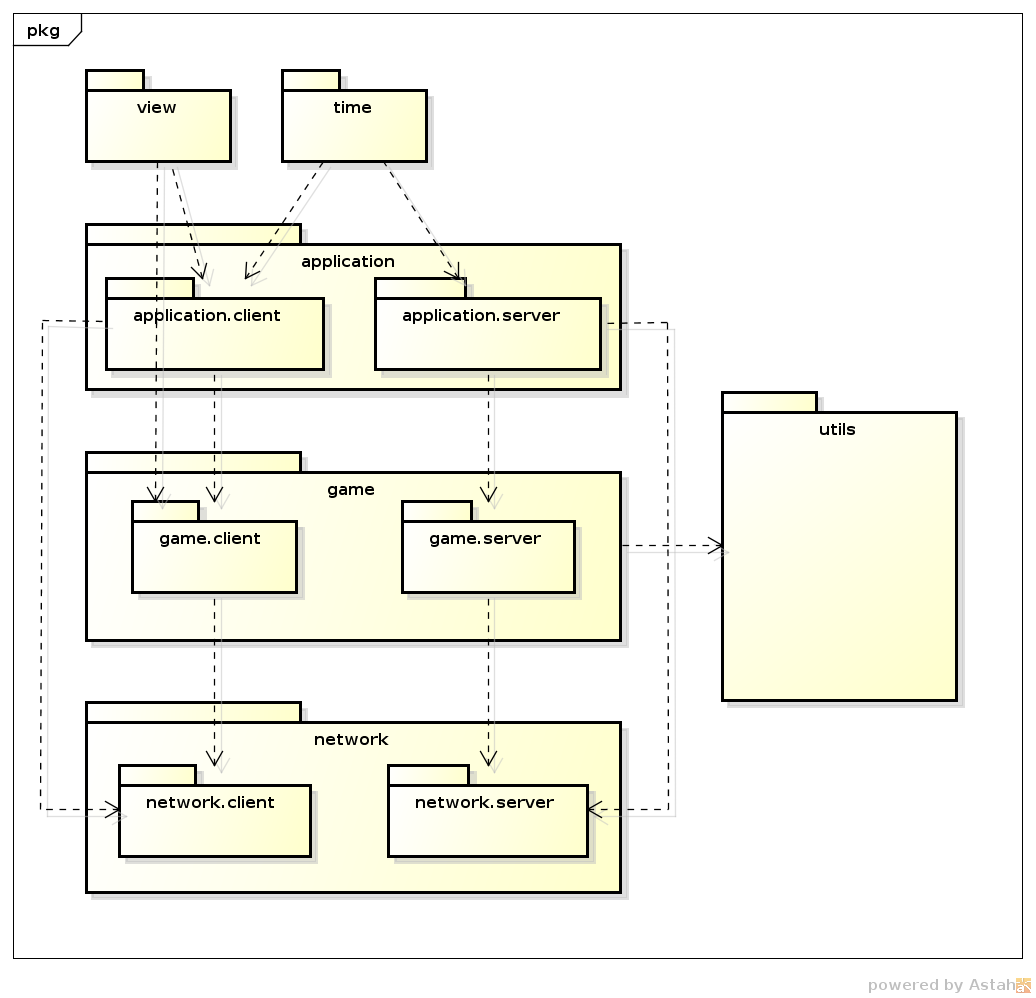
\includegraphics[scale=0.5]{LogischeSicht}

\newpage

\subsection{ <Presentation/view>}
Im Package view befinden sich Frames und Canvas, die für die Presentation des Clients notwendig sind.


\subsubsection{Klassenstruktur}
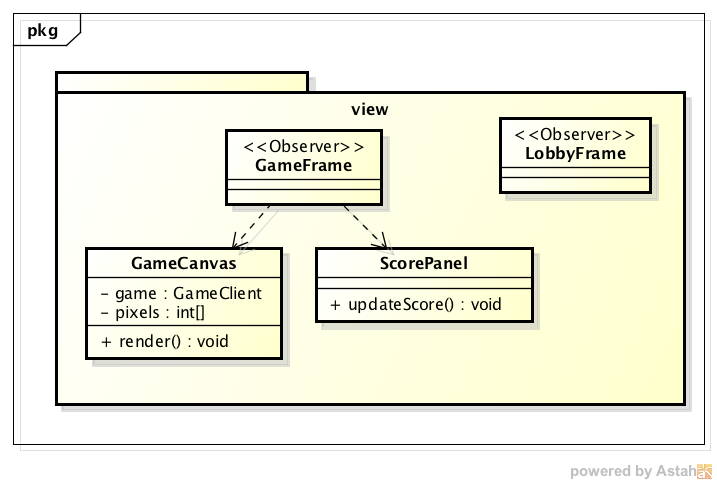
\includegraphics[scale=0.8]{ClassDiagramView}


\textbf{GameFrame}\\
Der GameFrame ist ein Observer und delegiert die Notifies an das zugehörige Panel, die sich dann selber auf den neusten Stand bringen.\\\\

\textbf{GameCanvas}\\
Der GameCanvas kümmert sich nur um das Rendering, also das Zeichnen der Szene. Dabei delegiert er jedoch nur die pixels[] an alle Sprites, welche sich dann eigenständig zeichnen. Der GameCanvas kümmert sich dann um das performante Buffering.\\\\
\begin{tabularx}{\linewidth}{l p{12cm}}
\textbf{Methode} & \textbf{Beschreibung}\\
\hline
render():void & Kümmert sich um die BufferStrategy und delegiert das zeichnen der Sprites direkt an die Sprites selbst.
\end{tabularx}

\newpage

\subsubsection{Wichtige interne Abläufe}
<Beschreibung von wichtigen internen Abläufen>


\subsection{Wichtige Abläufe}
<Beschreibung von wichtigen Abläufen (packageübergreifend)>
 
\section{Prozesse und Threads}
<Wenn mehrere Prozesse oder Threads eingesetzt werden wird hier beschrieben, wie diese ablaufen, miteinander funktionieren, Daten austauschen, sich synchronisieren, usw.>
 
\section{Deployment}
<Beschreibung der einzelnen Komponenten und deren Aufteilung (auf welchen Umgebungen, Servern, usw. laufen die Komponenten)>
 
\section{Datenspeicherung}
<Beschreibung mit Diagramm der Datenspeicherung (Datenmodell, z.B. Datenbank)>
 
\section{Grössen und Leistung}
<Einschränkungen der Applikation bezüglich Speicher, Leistung, etc…. (zum Beispiel: Verwaltung unterstützt maximal 20'000 Einträge)>


\end{document}